\documentclass[10pt]{article}
\usepackage[preprint]{tmlr}
\input{math_commands.tex}

\usepackage{hyperref}
\usepackage{url}
\usepackage{doi}
\usepackage{graphicx}
\usepackage{booktabs}
\usepackage{xcolor}
\usepackage{float}

\title{Project Proposal: Visualizing Global CO\textsubscript{2} Emissions and Climate Accountability\\
\large COMP 6934 -- Introduction to Data Visualization, Winter 2026}

\author{\name Isaac Edem Adoboe (202384695) \email ieadoboe@mun.ca \\
      \addr Department of Mathematics and Statistics\\
      Memorial University of Newfoundland}

\def\month{02}
\def\year{2026}
\def\openreview{\url{https://openreview.net/forum?id=XXXX}}

\begin{document}
\maketitle

\begin{abstract}
This proposal describes a visualization project exploring global CO\textsubscript{2} emissions, historical responsibility, and economic decoupling using the Our World in Data CO\textsubscript{2} and Greenhouse Gas Emissions dataset (50{,}411 rows, 79 attributes, 254 countries, 1750--2024). Four interactive visualizations are proposed: (1) a proportional symbol map showing cumulative historical responsibility against current per-capita emissions; (2) small-multiple line charts decomposing national emissions by fuel source over time; (3) an annotated scatterplot contrasting production-based and consumption-based emissions to reveal emissions outsourcing; and (4) a connected scatterplot tracing each country's trajectory through economic growth and emissions space. The project targets climate policy analysts who need to assess national accountability, benchmark transition progress, and communicate emissions trajectories to policymakers.
\end{abstract}

%% ============================================================
\section{Introduction}
\label{sec:intro}

Who is responsible for global CO\textsubscript{2} emissions? The answer depends on how the question is framed: by historical accumulation, by consumption rather than production, by the pace of decarbonization, or by the fuel sources driving emissions. Each framing reveals a different accountability story. This project uses a single rich longitudinal dataset to build four visualizations that address these framings in sequence, targeting non-specialist policymakers who need to act on the results.

\subsection{Dataset}

\textbf{OWID CO\textsubscript{2} and Greenhouse Gas Emissions Dataset} (\texttt{owid-co2-data.csv}): 50{,}411 rows $\times$ 79 columns, covering 254 countries from 1750--2024. Annual data includes CO\textsubscript{2} emissions by fuel type (coal, oil, gas, cement, flaring, land-use change), production-based and consumption-based emissions, cumulative emissions, per-capita and GDP-intensity metrics, and socioeconomic indicators (GDP, population). The dataset is maintained by Our World in Data under CC BY 4.0 and draws on the Global Carbon Budget (Friedlingstein et al.), Jones et al.\ national contributions to climate change, the Energy Institute Statistical Review of World Energy, and the World Bank.

\subsection{Client}

The client is a senior policy analyst at an intergovernmental climate accountability body --- such as the IPCC Working Group III technical support unit or Environment and Climate Change Canada --- advising negotiators on emissions responsibility, transition benchmarking, and climate finance allocation. The analyst needs to: (a) identify which countries bear the greatest historical emissions burden; (b) determine whether high-income countries are genuinely decarbonizing or outsourcing emissions; (c) assess whether national fuel-source transitions are producing real reductions; and (d) compare countries across emissions and development dimensions to target bilateral cooperation.

%% ============================================================
\section{Preliminary Data Analysis (\emph{What})}
\label{sec:what}

\subsection{Dataset Types}

The dataset is a \textbf{flat table} of 50{,}411 items (country-year observations) across 79 attributes, keyed by (\texttt{country}, \texttt{year}). It is \textbf{temporal}: \texttt{year} is an ordered sequential key from 1750 to 2024, sparse before 1850 and near-complete from 1990 onward. It is \textbf{spatial} in the sense that countries are identified by ISO code and can be mapped to geographic coordinates, though no geometry is embedded in the data.

\subsection{Attribute Types}

Table~\ref{tab:attributes} classifies the key attributes. Three distinctions matter for channel selection. \textbf{Sequential} quantitative attributes (e.g., \texttt{co2}, \texttt{gdp}) have a natural zero and increase in one direction; they suit single-hue colormaps and proportional encodings. \textbf{Diverging} quantitative attributes (e.g., \texttt{land\_use\_change\_co2}) have a meaningful midpoint at zero, with positive values indicating net carbon sources and negative values indicating net sinks; they require a diverging colormap anchored at zero. \textbf{Ordered categorical} attributes (e.g., income group: Low $<$ Lower-middle $<$ Upper-middle $<$ High) have a natural rank but no numeric distance; they suit an ordinal sequential palette rather than a nominal one.

\begin{table}[h]
\caption{Key attributes and their Munzner types.}
\label{tab:attributes}
\begin{center}
\begin{tabular}{lllll}
\toprule
\textbf{Attribute} & \textbf{Type} & \textbf{Subtype} & \textbf{Order} & \textbf{Role} \\
\midrule
\texttt{country}                      & Categorical  & Nominal   & Unordered  & Key \\
\texttt{year}                         & Quantitative & Ordered   & Sequential & Key \\
\texttt{iso\_code}                    & Categorical  & Nominal   & Unordered  & Geographic lookup \\
\texttt{population}                   & Quantitative & Sequential & Sequential & Size encoding \\
\texttt{gdp}                          & Quantitative & Sequential & Sequential & Economic indicator \\
\texttt{co2}                          & Quantitative & Sequential & Sequential & Territorial emissions \\
\texttt{co2\_per\_capita}             & Quantitative & Sequential & Sequential & Per-person burden \\
\texttt{co2\_per\_gdp}                & Quantitative & Sequential & Sequential & Carbon intensity \\
\texttt{cumulative\_co2}              & Quantitative & Sequential & Sequential & Historical responsibility \\
\texttt{consumption\_co2}             & Quantitative & Sequential & Sequential & Consumption-based emissions \\
\texttt{consumption\_co2\_per\_capita}& Quantitative & Sequential & Sequential & Consumption burden \\
\texttt{coal\_co2}                    & Quantitative & Sequential & Sequential & Fuel-source decomposition \\
\texttt{oil\_co2}                     & Quantitative & Sequential & Sequential & Fuel-source decomposition \\
\texttt{gas\_co2}                     & Quantitative & Sequential & Sequential & Fuel-source decomposition \\
\texttt{cement\_co2}                  & Quantitative & Sequential & Sequential & Fuel-source decomposition \\
\texttt{flaring\_co2}                 & Quantitative & Sequential & Sequential & Fuel-source decomposition \\
\texttt{land\_use\_change\_co2}       & Quantitative & Diverging  & Diverging  & Fuel-source decomposition \\
\texttt{temperature\_change\_from\_co2}& Quantitative& Sequential & Sequential & Climate impact \\
income group (derived)                & Categorical  & Ordered   & Ordinal    & Grouping \\
continent (derived)                   & Categorical  & Nominal   & Unordered  & Grouping \\
\bottomrule
\end{tabular}
\end{center}
\end{table}

\subsection{Data Sufficiency}

The dataset exceeds sufficiency requirements on all dimensions. Quantity: 50{,}411 rows across 274 years. Diversity: 79 attributes spanning sequential, diverging, ordered categorical, and nominal types, supporting a wide range of mark and channel combinations. Completeness: for the primary analysis window (1990--2022), \texttt{co2} and fuel-type breakdowns exceed 95\% completeness for countries covering over 99\% of global emissions; \texttt{consumption\_co2} reaches approximately 85\% for 1990--2018; \texttt{gdp} and \texttt{population} are complete for all countries of analytical interest.

%% ============================================================
\section{Client Questions (\emph{Why})}
\label{sec:why}

\subsection{Question 1: Which countries are outliers in the relationship between cumulative historical CO\textsubscript{2} responsibility and current per-capita emissions?}

Countries that contributed most to the atmospheric CO\textsubscript{2} stock are not necessarily those with the highest per-capita emissions today. The analyst needs to identify which countries occupy anomalous positions in this space: historically large emitters that have reduced output, or modest historical contributors with rapidly rising current emissions. This question is broad by design, covering all countries and the full dataset span, leaving room for the visualization to reveal unexpected patterns.

\textbf{Munzner \emph{why}}: 

\textit{Primary}: \textsc{Query} $\rightarrow$ \textbf{Identify} outliers in the dependency between \texttt{cumulative\_co2} and \texttt{co2\_per\_capita}.


\textit{Secondary}: \textsc{Query} $\rightarrow$ \textbf{Extremes} (which countries have the largest cumulative totals?).

\subsection{Question 2: What trend characterizes the fuel-source composition of major emitters over time, and are structural transitions detectable?}

The analyst needs to know whether a sustained directional shift --- a narrowing coal stream, a rising gas contribution, a shrinking land-use-change component --- is visible in the data. This question is more specific than Question~1, targeting the six fuel-type decomposition attributes directly and asking a directional question about change. It leaves design room in how the decomposition is encoded and how countries are compared.

\textbf{Munzner \emph{why}}: 

\textit{Primary}: \textsc{Analyze} $\rightarrow$ \textbf{Discover} the trend in fuel-source composition (\texttt{coal\_co2}, \texttt{oil\_co2}, \texttt{gas\_co2}, \texttt{cement\_co2}, \texttt{flaring\_co2}, \texttt{land\_use\_change\_co2}) over time.

\textit{Secondary}: \textsc{Compare} $\rightarrow$ \textbf{Features} (do different emitters exhibit different transition shapes?).

\subsection{Question 3: Is there a systematic correlation between income group and emissions outsourcing, measured by the gap between production-based and consumption-based CO\textsubscript{2} per capita?}

This question targets a politically consequential accountability gap: whether wealthy nations' territorial emissions reductions reflect genuine decarbonization or the offshoring of carbon-intensive production. It is the most attribute-specific of the three, directing attention to \texttt{co2\_per\_capita}, \texttt{consumption\_co2\_per\_capita}, and the derived ordered categorical \texttt{income\_group}. A reference condition --- production equals consumption --- can be encoded directly into the visualization geometry, making the question unusually well-suited to a specific design.

\textbf{Munzner \emph{why}}: 

\textit{Primary}: \textsc{Query} $\rightarrow$ \textbf{Identify} the correlation between \texttt{income\_group} (ordered categorical) and deviation from the production--consumption neutrality condition.

\textit{Secondary}: \textsc{Query} $\rightarrow$ \textbf{Outliers} (which specific countries deviate most?).

%% ============================================================
\section{Proposed Visualizations (\emph{How})}
\label{sec:how}

\subsection{Visualization 1: Proportional Symbol Map}

\textbf{Goal}: Identify outlier countries in the joint space of cumulative historical CO\textsubscript{2} burden and current per-capita emissions, with geographic context.

\textbf{Idiom}: A world map with one point mark per country, positioned at the country's geographic centroid. Bubble area encodes \texttt{cumulative\_co2} (sequential quantitative) using a proportional symbol scaling. Bubble color encodes \texttt{co2\_per\_capita} on a perceptually uniform single-hue sequential colormap. A year dropdown (default: 2022) controls which year's per-capita value is shown; the cumulative total updates accordingly. Hovering reveals country name, cumulative total, per-capita value, and year.

The key design insight is dual temporal encoding in a single frame: bubble area accumulates historically while bubble color reflects the current year selected. This makes the accountability gap large historical burden, low current emissions, or vice versa legible without a second chart or animation.

\textbf{Marks and channels}: Point marks on a geographic base. Area $\rightarrow$ \texttt{cumulative\_co2} (sequential). Color luminance $\rightarrow$ \texttt{co2\_per\_capita} (sequential). Geographic position $\rightarrow$ country centroid (spatial).

\textbf{\emph{How} elements}: \textsc{Encode} (area, color, position); \textsc{Manipulate} (year dropdown, hover tooltip); \textsc{Reduce} (filter to countries with valid \texttt{iso\_code}; clip bubble radii at 99th percentile; enforce minimum visible radius).

\textbf{Design note}: Bubble area is a lower-ranked channel than position for magnitude judgment. The hover tooltip compensates by providing exact values. Bubbles are sized to make the largest emitters immediately prominent while keeping smaller countries visible --- the primary task is outlier identification, not precise magnitude reading.

\textbf{Relation to questions}: Directly addresses Question~1. The geographic base adds spatial pattern recognition (regional clusters of large historical emitters) not available in a non-geographic design.

\subsection{Visualization 2: Small-Multiple Line Charts}

\textbf{Goal}: Discover whether major emitters show a structural trend away from high-carbon fuel sources over time.

\textbf{Idiom}: A small-multiple panel of 8 line charts (USA, China, Russia, India, Germany, UK, Japan, Brazil), one per country, each showing one line per fuel source (\texttt{coal\_co2}, \texttt{oil\_co2}, \texttt{gas\_co2}, \texttt{cement\_co2}, \texttt{flaring\_co2}) from 1950 to 2022. All panels share the same x-axis (year) and a common y-axis scale (MtCO\textsubscript{2}), enabling direct cross-country magnitude comparison. A consistent categorical color palette for fuel types is applied across all panels. \texttt{land\_use\_change\_co2}, being a diverging attribute, is rendered separately within each panel with a zero-baseline reference line and a diverging color treatment distinguishing source years from sink years. Policy milestones (Kyoto 1997, Paris 2016) are marked as vertical reference lines across all panels. A country dropdown allows the analyst to substitute any of the 254 countries into a full-resolution single-panel view.

\textbf{Marks and channels}: Line marks. Horizontal position $\rightarrow$ \texttt{year} (sequential). Vertical position $\rightarrow$ emissions magnitude (MtCO\textsubscript{2}, sequential). Color hue $\rightarrow$ fuel type (nominal categorical, consistent across panels). Spatial region (facet) $\rightarrow$ country identity.

\textbf{\emph{How} elements}: \textsc{Encode} (position, color); \textsc{Facet} (small multiples by country); \textsc{Manipulate} (country dropdown for single-panel deep-dive, hover tooltip); \textsc{Reduce} (3-year rolling mean on \texttt{land\_use\_change\_co2} to suppress pulse noise from forest-fire events, disclosed in subtitle).

\textbf{Design note}: Position encodes both time and magnitude on a zero baseline, giving accurate trend and magnitude reading for each fuel source independently. Sharing the y-axis scale across all small multiples preserves cross-country comparability at the cost of compressing lines for smaller emitters; the single-panel dropdown view resolves this for within-country analysis.

\textbf{Relation to questions}: Directly addresses Question~2. The small-multiple layout makes structural differences between countries immediately visible by spatial juxtaposition --- a coal-dominated and growing profile (China, India) reads differently from an oil-and-gas profile in decline (UK, Germany) without any interaction required.

\subsection{Visualization 3: Annotated Log-Log Scatterplot}

\textbf{Goal}: Identify whether emissions outsourcing --- consuming more carbon than is territorially produced --- is systematically correlated with income group.

\textbf{Idiom}: A scatterplot for a user-selected year (default: 2019, the most recent year with near-complete \texttt{consumption\_co2} coverage). X-axis: \texttt{co2\_per\_capita} (production-based, log scale). Y-axis: \texttt{consumption\_co2\_per\_capita} (demand-based, log scale). One point mark per country. Bubble size encodes \texttt{population}. Color encodes \texttt{income\_group} using an ordinal sequential palette (light to dark: Low to High income), preserving the ordered categorical structure. A diagonal reference line ($y = x$) encodes the neutrality condition: countries above consume more than they produce (net emissions importers); countries below produce more than they consume (net emissions exporters). Quadrant regions are annotated directly on the chart. Key outliers are labeled. A year slider allows the analyst to track how country positions have shifted since 1990.

\textbf{Marks and channels}: Point marks. Horizontal position $\rightarrow$ \texttt{co2\_per\_capita} (log, sequential). Vertical position $\rightarrow$ \texttt{consumption\_co2\_per\_capita} (log, sequential). Area $\rightarrow$ \texttt{population} (sequential). Color luminance $\rightarrow$ \texttt{income\_group} (ordinal sequential). Annotation text $\rightarrow$ country identity (outliers).

\textbf{\emph{How} elements}: \textsc{Encode} (position, size, color); \textsc{Annotate} (reference diagonal, quadrant labels, outlier labels); \textsc{Manipulate} (year slider, hover tooltip); \textsc{Reduce} (filter to countries with valid data in both attributes; log scale to prevent range compression).

\textbf{Design note}: The reference diagonal is not merely a visual aid --- it encodes a normative claim about accountability directly into the geometry of the chart. The ordinal sequential palette for income group is a deliberate choice: a nominal palette would discard the income ordering that is central to the analytical question. Log axes are necessary given the four-order-of-magnitude range of per-capita emissions; the hover tooltip provides raw values for readers who find log scales unintuitive.

\textbf{Relation to questions}: Directly addresses Question~3. Also provides the consumption-side evidence that contextualizes the decoupling analysis in Visualization~4: a country may show falling production-based emissions while its consumption-based footprint remains high.

\subsection{Visualization 4: Connected Scatterplot}

\textbf{Goal}: Discover whether a country's CO\textsubscript{2} emissions trajectory has decoupled from its economic growth trajectory, and characterize the shape of that decoupling over time.

\textbf{Idiom}: A connected scatterplot for a user-selected country (default: Germany) and time window (default: 1990--2022). X-axis: GDP per capita (\texttt{gdp} divided by \texttt{population}), encoding economic prosperity. Y-axis: \texttt{co2\_per\_capita}, encoding emissions intensity. One point per year, connected by a path in chronological order, with year labels at regular intervals. The path is colored by year using a sequential colormap (light to dark) to reinforce temporal direction. Directional arrows mark the path at several points.

The decoupling argument is encoded directly in the geometry: a path that moves rightward (rising GDP per capita) while simultaneously moving downward (falling CO\textsubscript{2} per capita) traces a southeast trajectory --- the geometric signature of absolute per-capita decoupling. A horizontal reference at the starting-year CO\textsubscript{2} value marks the threshold below which absolute decoupling has occurred. Countries still growing in both dimensions trace a northeast path; those contracting in both trace a southwest path.

\textbf{Marks and channels}: Point marks (one per year). Line marks (connecting consecutive years). Horizontal position $\rightarrow$ GDP per capita (sequential). Vertical position $\rightarrow$ \texttt{co2\_per\_capita} (sequential). Color luminance $\rightarrow$ year (sequential). Text annotation $\rightarrow$ year labels.

\textbf{\emph{How} elements}: \textsc{Encode} (position for both key attributes, color for time); \textsc{Annotate} (year labels, directional arrows, horizontal decoupling threshold); \textsc{Manipulate} (country dropdown, time window slider, hover for exact year values); \textsc{Reduce} (filter to years with complete \texttt{gdp}, \texttt{co2}, and \texttt{population}; linear interpolation for short isolated gaps).

\textbf{Design note}: The connected scatterplot places both key attributes on position axes --- the highest-ranked channel for quantitative data --- rather than requiring the analyst to mentally overlay two separate time series. The decoupling argument is visible as a geometric direction, not as a gap between lines. The path can become visually complex for countries with non-monotonic trajectories (e.g., post-Soviet economies); year labels and directional arrows are essential for legibility in these cases.

\textbf{Relation to questions}: Synthesizes all three client questions. It shows whether a historically large emitter (Question~1) is genuinely reducing per-capita output, whether fuel-source transitions (Question~2) are translating into aggregate reductions, and provides the production-side complement to the outsourcing analysis (Question~3).

\subsection{Mockup Charts}

\begin{figure}[H]
\centering
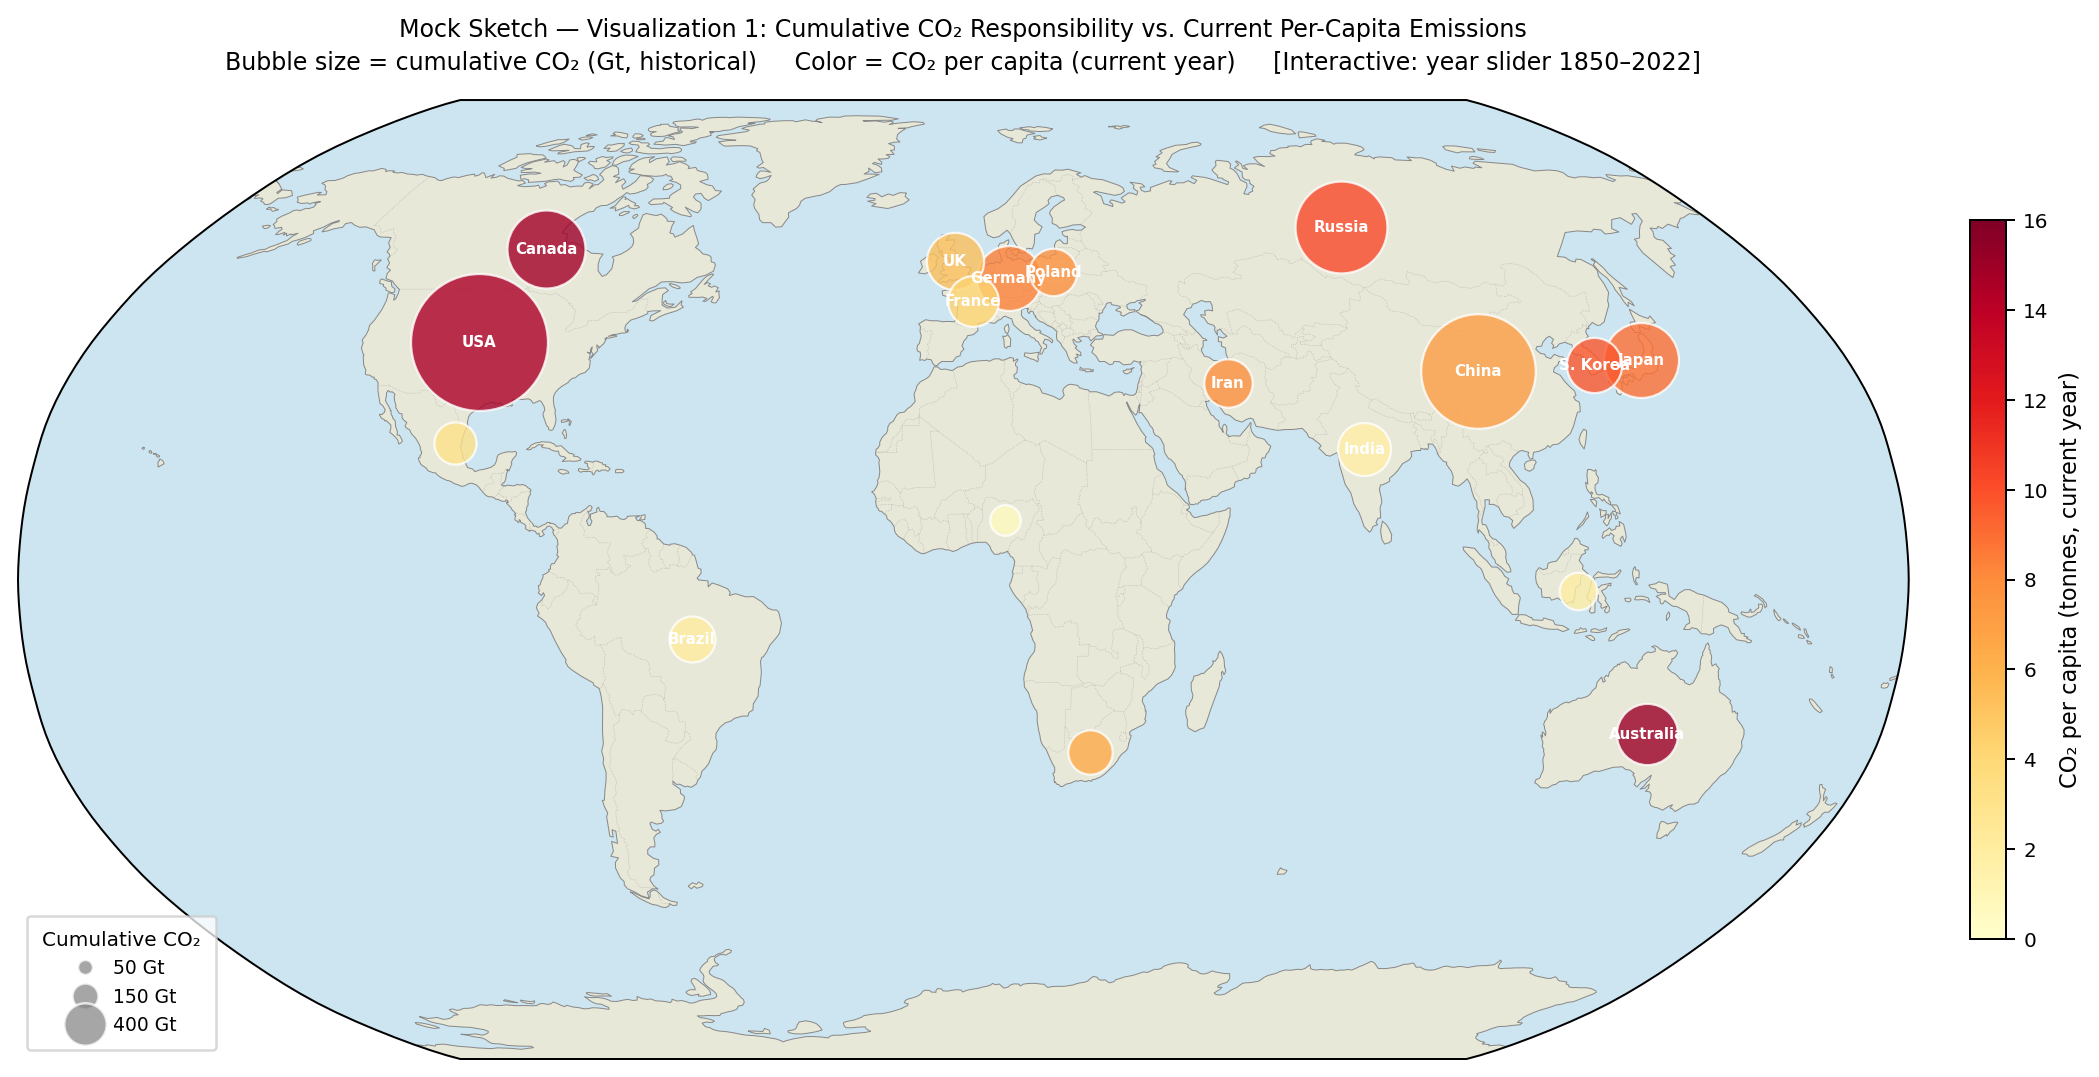
\includegraphics[width=0.9\linewidth]{viz1_bubble_map.png}
\caption{Visualization 1 (mock sketch) - Proportional Symbol Map. Bubble area encodes \texttt{cumulative\_co2}; color encodes \texttt{co2\_per\_capita} for the selected year.}
\label{fig:viz1}
\end{figure}

\begin{figure}[H]
\centering
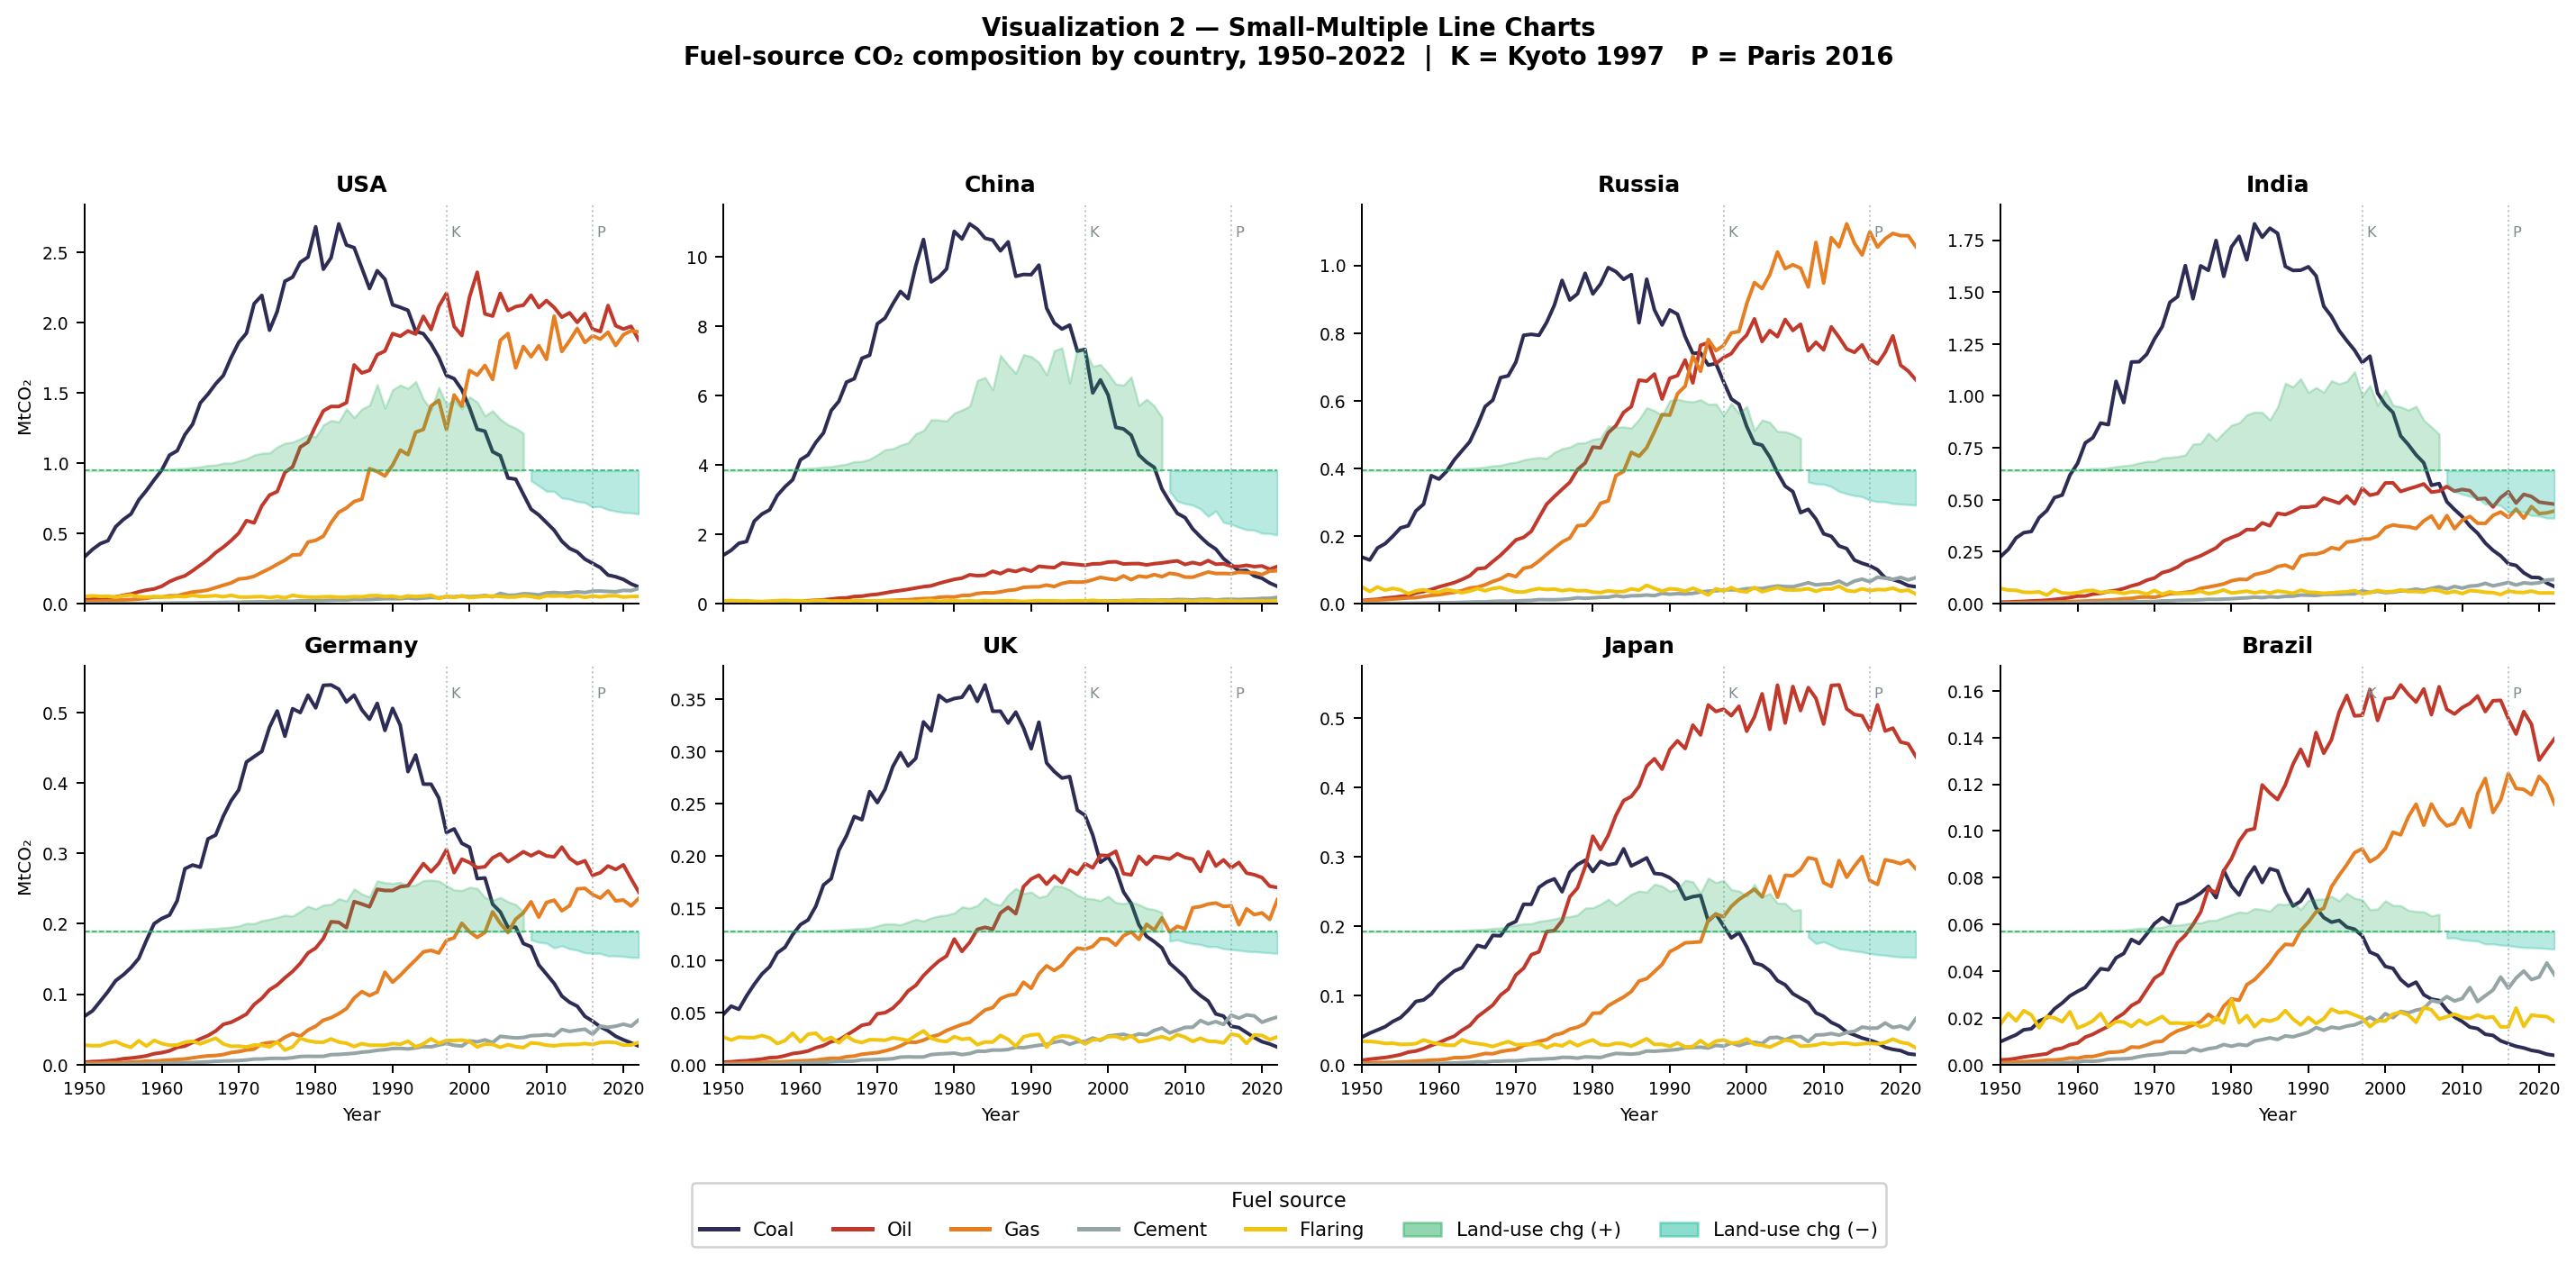
\includegraphics[width=\linewidth]{viz2_linechart.png}
\caption{Visualization 2 (mock sketch) --- Small-Multiple Line Charts. One panel per major emitter; one line per fuel source; shared axes enable cross-country comparison.}
\label{fig:viz2}
\end{figure}

\begin{figure}[H]
\centering
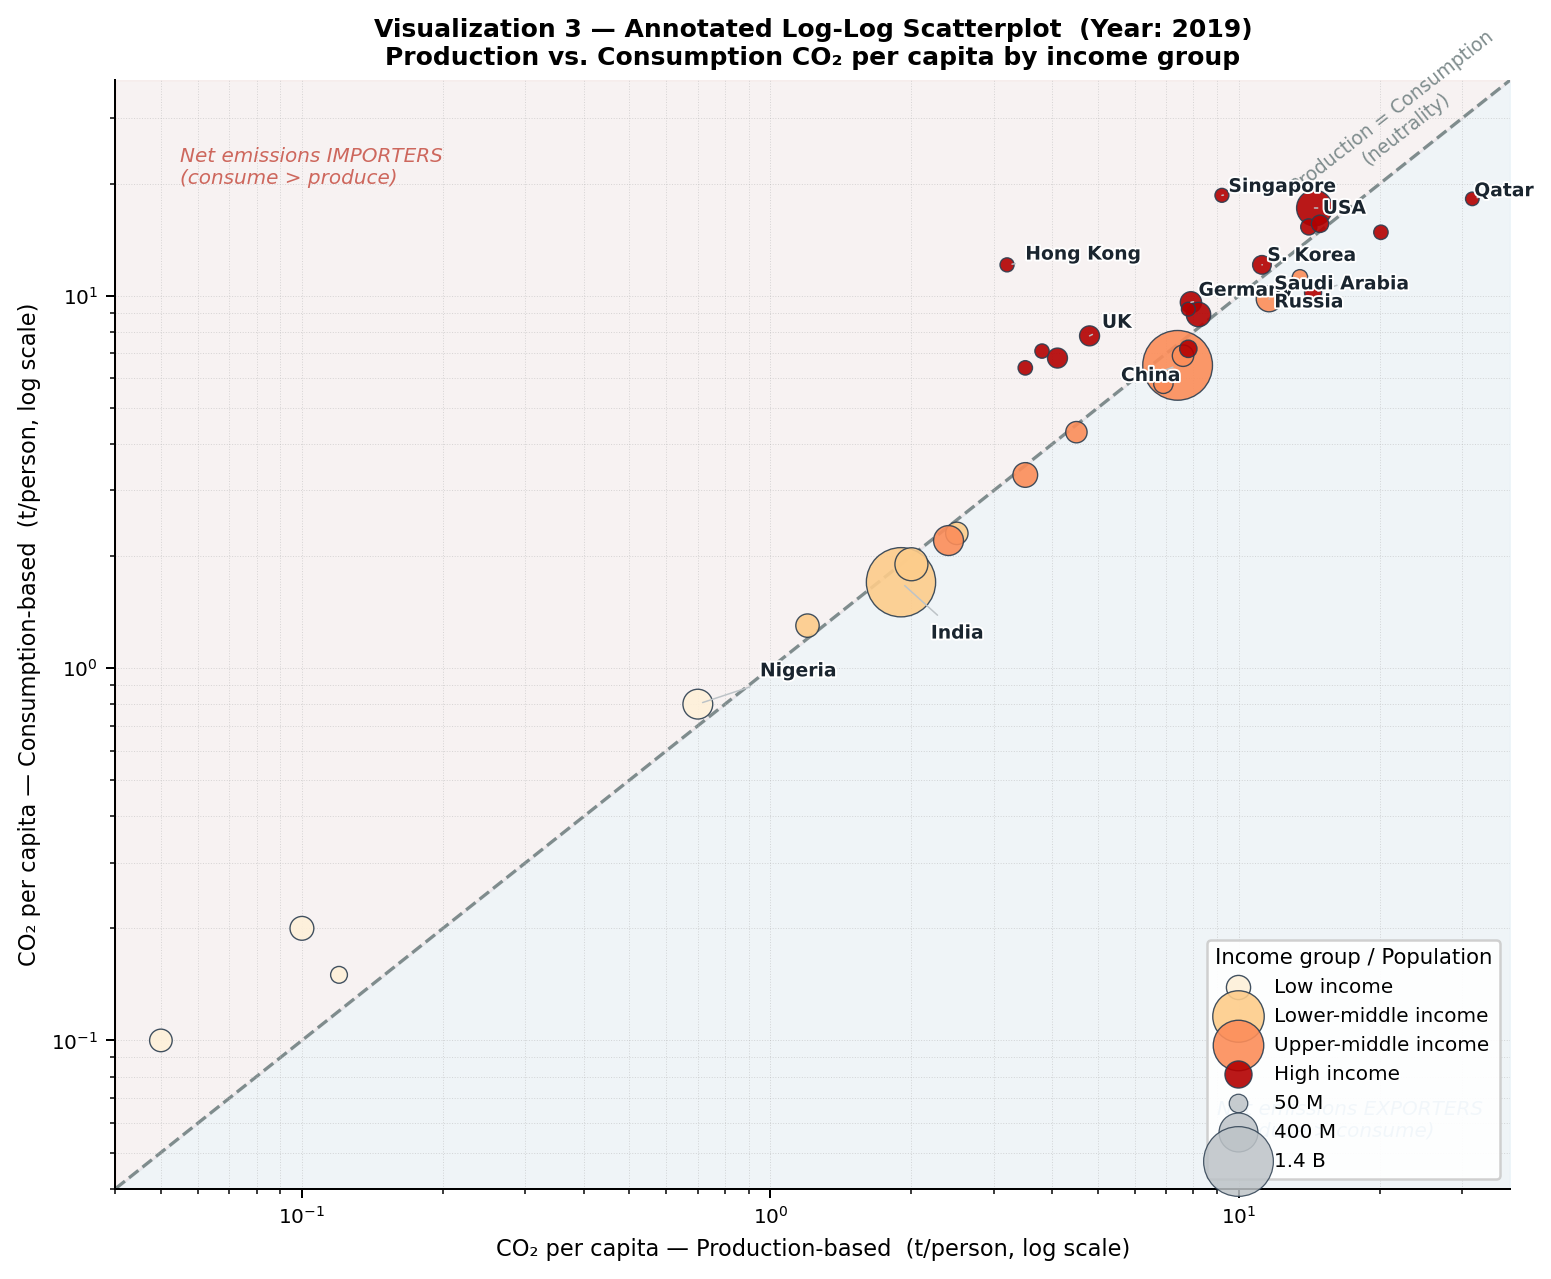
\includegraphics[width=0.7\linewidth]{viz3_scatter.png}
\caption{Visualization 3 (mock sketch) --- Annotated Log-Log Scatterplot. Reference diagonal encodes the production--consumption neutrality condition. Color encodes income group (ordinal sequential palette).}
\label{fig:viz3}
\end{figure}

\begin{figure}[H]
\centering
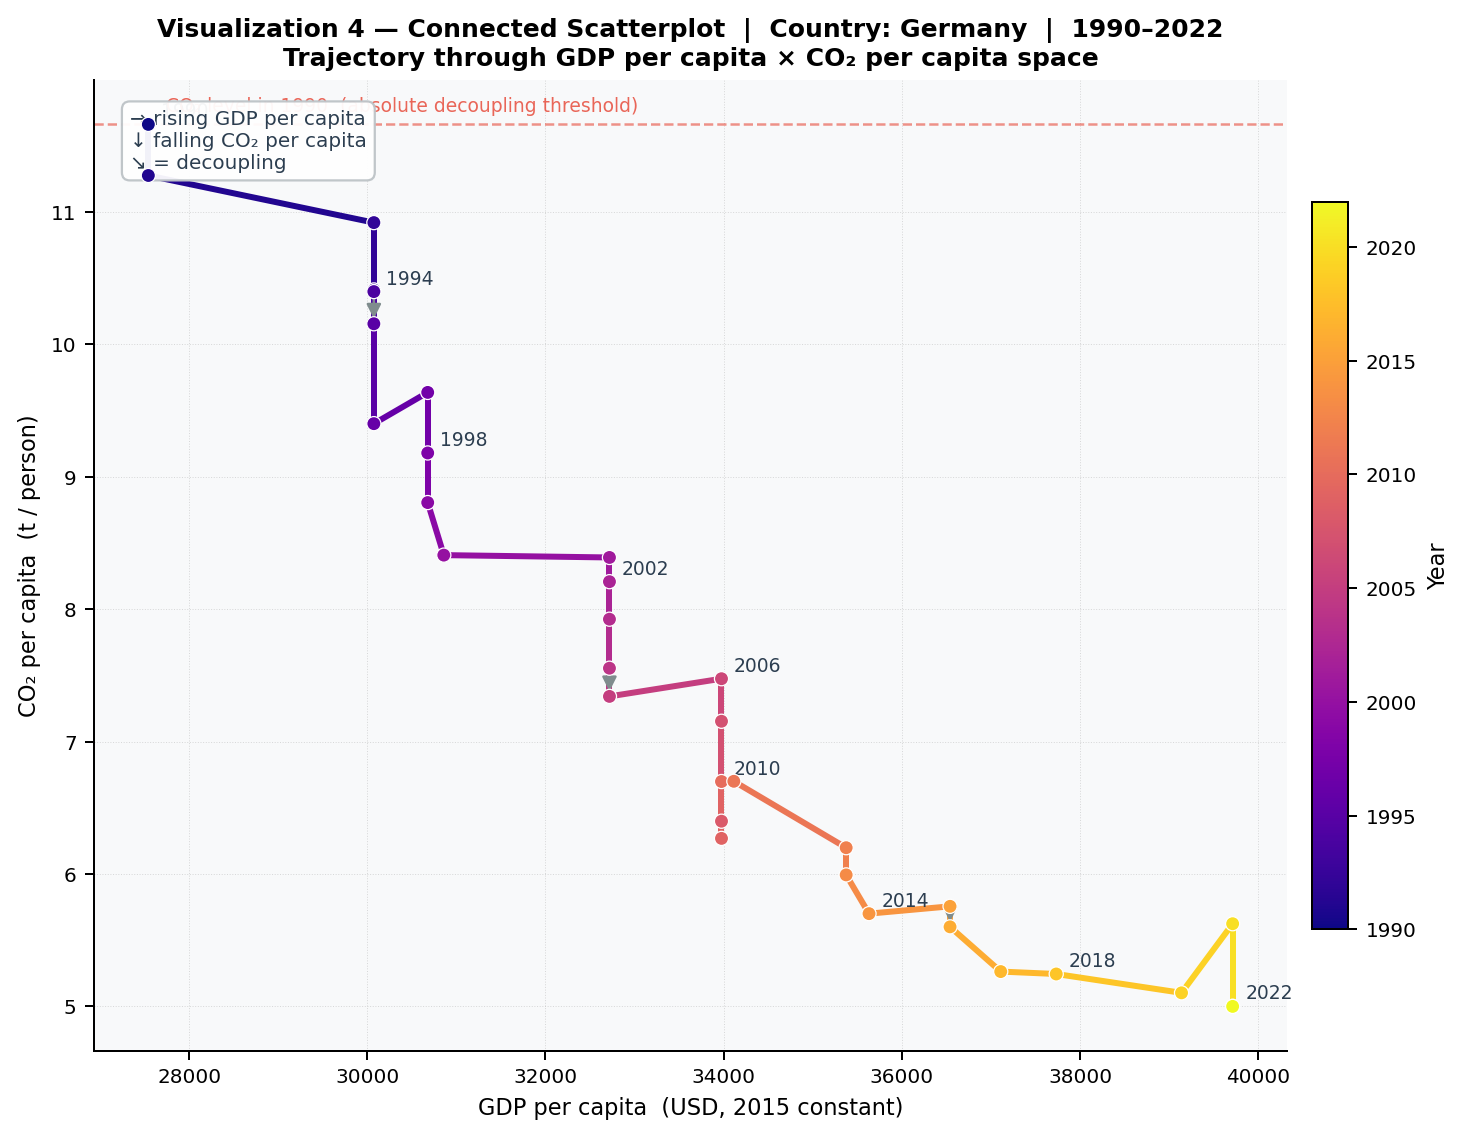
\includegraphics[width=0.7\linewidth]{viz4_decoupling.png}
\caption{Visualization 4 (mock sketch) --- Connected Scatterplot. Each point is one year; the path direction encodes the decoupling trajectory through GDP-per-capita vs.\ CO\textsubscript{2}-per-capita space.}
\label{fig:viz4}
\end{figure}

\newpage
%% ============================================================
\section*{Attributions}

\textbf{Dataset}: Hannah Ritchie, Pablo Rosado, Edouard Mathieu, and Max Roser (2023). ``CO\textsubscript{2} and Greenhouse Gas Emissions.'' Published online at \url{OurWorldInData.org}. Retrieved from \url{https://github.com/owid/co2-data}. Licensed under CC BY 4.0. The dataset draws on the Global Carbon Budget (Friedlingstein et al.), Jones et al.\ (2024), the Energy Institute Statistical Review of World Energy, the U.S.\ Energy Information Administration, the World Bank, Gapminder, and the UN World Population Prospects.

\textbf{Tools}: Pandas, NumPy, Matplotlib.

\textbf{Mockup charts}: Generated using \texttt{matplotlib} with synthetic data produced by feeding the dataset's attribute names into ChatGPT. They are illustrative only and do not reflect the actual data.

\end{document}